\begin{song}{title=\centering What Shall We Do With the Drunken Sailor \\\normalsize   \vspace*{-0.3cm}}  %% sem se napíše jméno songu a autor
\moveright 4.8cm \vbox{      %Varianta č. 1  ---> Jeden sloupec zarovnaný na střed	

\sloka 
	^{Dmi}What shall we do with a drunken sailor 
	
	^{C\,{\color{white}\_}}what shall we do with a drunken sailor 

	^{Dmi}what shall we do with a drunken sailor 
	
	^{F{\color{white}\_}}early ^{A7}in the ^{Dmi{\color{white}\_\_\_}}morning? 


\refren
	^{Dmi{\color{white}\_}}Hooray and up she rises ^{C{\color{white}\_\_}}hooray and up she rises 
	
	^{Dmi{\color{white}\_}}hooray and up she rises ^{F{\color{white}\_}}early ^{A7}in the ^{Dmi{\color{white}\_\_}}morning. 


\sloka
	/: Put him in the longboat till he's sober :/ (3x)

	early in the morning. 


\refren

\sloka
	/: Pull out the plug and wet him all over :/ (3x)
	
	early in the morning. 

\refren

\sloka
	/: Put him in the scuppers with hose-pipe on him :/ (3x)
	
	early in the morning. 

\refren

\sloka
	/: Heave him by the leg in running bowline :/ (3x)
	
	early in the morning. 

\refren

\sloka
	/: Tie him to the taffrail when she's yardarm under :/ (3x)
	
	early in the morning. 

\refren

}
\setcounter{Slokočet}{0}
\end{song}


\begin{figure}[h]
\centering
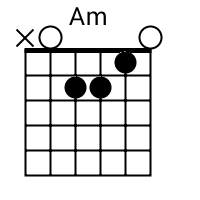
\includegraphics[scale=1.5]{../Akordy/am.png}
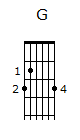
\includegraphics[scale=1.5]{../Akordy/g.png}
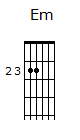
\includegraphics[scale=1.5]{../Akordy/em.png}
\end{figure}
